\documentclass[12pt]{article}
\usepackage{amsmath,amssymb,amsthm}
\usepackage[english]{babel}
\usepackage[utf8]{inputenc}
\usepackage{fancyhdr}
\usepackage{changepage} 

\usepackage{hyperref}

% for line spacing
\usepackage{setspace}

% for absolute value
\usepackage{commath}

% for numbering
\usepackage{enumerate}

% for image placing
\usepackage{float}

% paper size and margins
\usepackage[letterpaper, left=20mm, right=20mm, top=25mm, bottom = 25mm, headsep=.15in]{geometry}

% for curly brace
\usepackage{amsmath}

% for input images
\usepackage{graphicx}
\graphicspath{ {./} }
\usepackage{subfig}

% for printing pseudocode
\usepackage[boxed]{algorithm}
\usepackage[noend]{algpseudocode}

% for tables
\usepackage{tabularx}

\makeatletter
\def\BState{\State\hskip-\ALG@thistlm}
\makeatother

% for circled numbers
\usepackage{tikz}
\newcommand*\circled[1]{\tikz[baseline=(char.base)]{
            \node[shape=circle,draw,inner sep=1pt] (char) {#1};}}

% double line space
\renewcommand{\baselinestretch}{2.0}

% code highlighting
\usepackage{minted}

% header, footer and page number
\pagestyle{fancy}
\fancyhf{}
\rhead{Tiankai Jiang \quad 20834939}
\lhead{ECE657A \quad Assignment 3}
\fancyfoot[C]{\thepage}

\setlength{\headheight}{15pt}

\begin{document}
\noindent
{\LARGE The source code is at the end of this document}
\section{Classification: Feature Extraction + Classical Methods}
\subsection{Explanation of Design and Implementation Choices of your Model}
The models I used on Kaggle are XGBoost, SVM, Random Forest and Hist Gradient Boosting. Below is the procedure to show why I chose them.

Dataset was given with labels, so naturally supervised learning methods were considered. There are 784 dimensions in the dataset, therefore, PCA should be applied on it to extract the main features and to decrease the dimension. First I used standard scalar to centralize data and then drew the scree plot with top 100 principle components.
\begin{figure}[H]
\begin{center}
    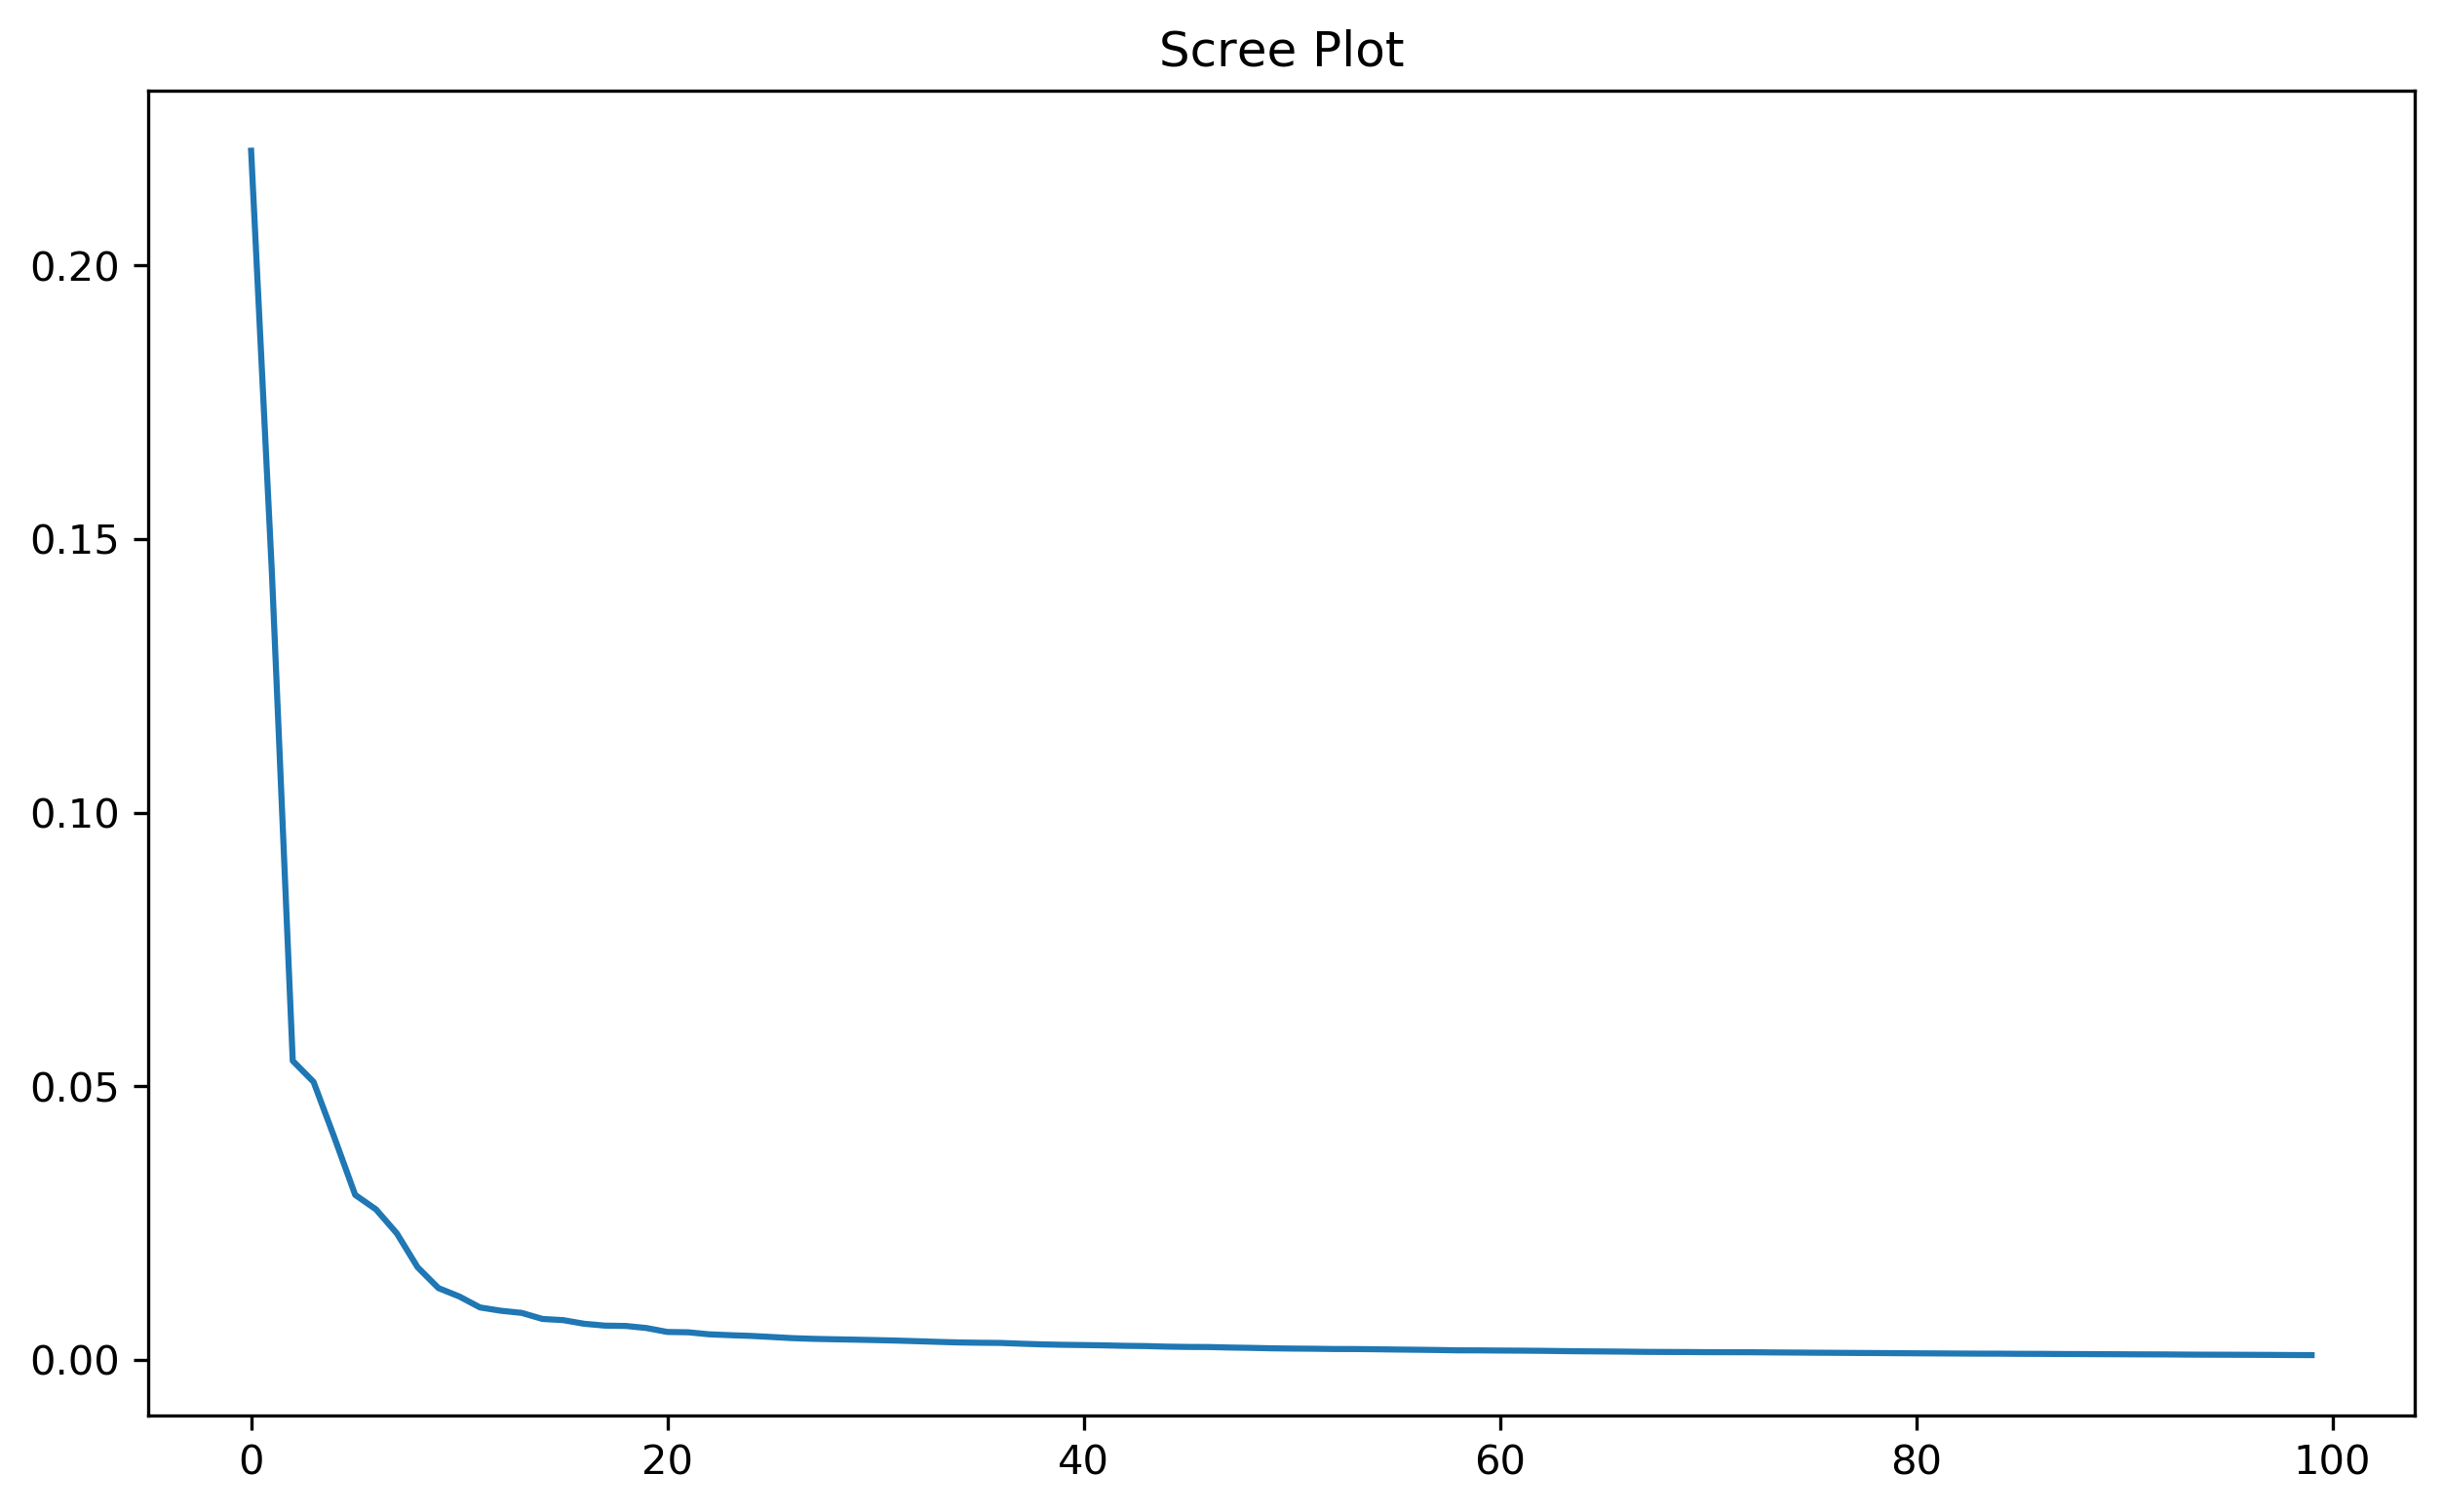
\includegraphics[width=0.7\textwidth]{./plots/ScreePlot.png}
\end{center}
\end{figure}
More than 99 percent of variance can be explained by the top 20 principle components. I took n\_components = 30 for a better result.

The following classification methods with default parameters were applied on the PCA transformed data. (Except for MultinomialNB since Naive Bayes based on applying Bayes' theorem with strong independence assumptions between the features, and preprocessing will seriously impact the result.) Using 20 percent data as test set, their corresponding accuracy are shown below.
\begin{center}
\begin{tabularx}{0.8\textwidth} { 
| >{\raggedright\arraybackslash}X 
| >{\raggedleft\arraybackslash}X | }
\hline
\textbf{Classifier} & \textbf{Accuracy}\\ 
\hline
MultiNomialNB & 47.18\%\\ 
\hline
Random Forest & 86.95\%\\ 
\hline
KNN & 85.86\%\\ 
\hline
SVM & 86.13\%\\
\hline
Logistic Regression & 67.78\%\\
\hline
LDA & 63.68\%\\
\hline
AdaBoost & 61.03\%\\
\hline
XGBoost & 87.14\%\\
\hline
Histogram-based Gradient Boosting & 87.38\%\\
\hline
\end{tabularx}
\end{center}

I did not try Gradient Boosting because both XGBoost and Hist Gradient Boosting are significantly faster than it. E.g. In the Hist Gradient Boosting's \href{https://scikit-learn.org/stable/modules/ensemble.html#histogram-based-gradient-boosting}{User Guide}

\begin{quotation}
  These histogram-based estimators can be \textbf{orders of magnitude faster} than GradientBoostingClassifier and GradientBoostingRegressor when the number of samples is larger than tens of thousands of samples.
\end{quotation}

Random Forest, KNN, SVM, XGBoost and Hist Gradient Boosting were chosen for further parameter tuning. KNN's accuracy was always 1-2 percent lower than the others so I eliminated it as well. The working mechanism for the rest four classifiers are as follows:

\textbf{Random Forest}: uses a large number of uncorrelated individual decision trees, and each tree will give a class prediction. The class with the most votes will be the model's final prediction.

\textbf{SVM}: applies a kernel function on the data and finds hyperplanes to separate two classes, and picks the one that maximizes the margin. For multiclass problems like this one, the problem will be treated as multiple binary classifications(One-vs-All or One-vs-One).

\textbf{Extreme Gradient Boosting}: just like gradient boosting, xgboost builds multiple trees, and each tree is based on minimizing the loss of the previous tree. And the final prediction is based on the sum of the learning rate times the prediction of each tree. However, xgboost uses a different loss function and introduces other parameters to make the modeling more robust and faster.

\textbf{Histogram-based Gradient Boosting}: a new experimental implementation of gradient boosting trees in sklearn 0.21, no blog or paper currently explains its detailed implementation. According to documentation, it is inspired by LightGBM.

I chose the above algorithms because their performance is relatively good. And except for SVM, the other 3 are ensemble methods, which provide an extra degree of freedom in the classical bias/variance tradeoff and they are also unlikely to overfit. In addition, they are easy to run on multicores to save running time.

Apart from PCA alone as the data preprocessing method, I also tried histogram of oriented gradients(HOG) or HOG combined with PCA as data preprocessing according to \href{https://www.ijitee.org/wp-content/uploads/papers/v8i5/E3075038519.pdf}{this paper}. HOG counts occurrences of gradient orientation in each localized area of an image, so that classification methods such as SVM can use these info to make prediction. However, the accuracy is only about 62\%.

\subsection{Implementation of your Design Choices}

\begin{singlespacing}
\begin{itemize}
\item Read data, apply standard scaler and PCA and train test split:
\begin{minted}[linenos,tabsize=4,breaklines]{python}
df = pd.read_csv('train.csv').drop(columns=['Id'])
X_train_pca, X_test_pca, y_train, y_test = train_test_split(PCA(n_components= 30).fit_transform( StandardScaler().fit_transform( df.iloc[:,1:].values)), df.iloc[:,0], test_size=0.2)
\end{minted}

\item Grid search, take random forest as example:
\begin{minted}[linenos,tabsize=4,breaklines]{python}
X = PCA(n_components = 30).fit_transform( StandardScaler().fit_transform( df.iloc[:,1:]))
modelRFC = GridSearchCV(RandomForestClassifier(random_state=42), {'criterion':['gini', 'entropy'], 'max_features': ['auto', 'log2', 0.25, 0.5, 0.75], 'min_samples_split': [2, 4, 6, 8, 10], 'min_samples_leaf': [1, 3, 5], 'max_depth': [20, 40, 60]}, n_jobs = -1, verbose=10).fit(X, df.iloc[:,0])
pprint(modelRFC.cv_results_)
pprint(modelRFC.best_params_)
\end{minted}

\item Function to plot the confusion matrix
\begin{minted}[linenos,tabsize=4,breaklines]{python}
def cm_plot(cm, y_test, title):
    N = list(map(lambda clazz : sum(y_test == clazz), [*range(5)]))
    plt.figure(figsize=(7,5)) 
    c = plt.pcolormesh([cm[j, :] / N[j] for j in range(5)], vmin=0.0, vmax=1.0)
    plt.title(title)
    plt.colorbar()
    plt.ylabel('Actual')
    plt.xlabel('Predicted')
    plt.xticks(0.5 + np.arange(5), np.arange(5))
    plt.yticks(0.5 + np.arange(5), np.arange(5))
    c.update_scalarmappable()
    ax = c.axes
    for p, color, value in zip(c.get_paths(), c.get_facecolors(), c.get_array()):
        x, y = p.vertices[:-2, :].mean(0)
        ax.text(x, y, "%.2f" % value, ha="center", va="center", color=(0.0, 0.0, 0.0) if sum(color[:2] > 0.3) >= 2 else (1.0, 1.0, 1.0))
    return plt.show()
\end{minted}

\item Function to plot the ROC curve
\begin{minted}[linenos,tabsize=4,breaklines]{python}
def roc_plot(y_test, y_score, name):
    fpr, tpr, roc_auc = dict(), dict(), dict()
    for i in range(5):
        fpr[i], tpr[i], _ = roc_curve(y_test[:, i], y_score[:, i])
        roc_auc[i] = auc(fpr[i], tpr[i])

    plt.figure(figsize=(7,7))
    plt.plot([0, 1], [0, 1], 'k--')
    [plt.plot(fpr[i], tpr[i], label= 'Class ' + str(i) + ' ROC(area = %0.2f)' % roc_auc[i]) for i in range(5)]
    plt.xlim([-0.02, 1.0])
    plt.ylim([0.0, 1.02])
    plt.xlabel('False Positive Rate')
    plt.ylabel('True Positive Rate')
    plt.legend(loc="lower right")
    plt.title(name + ' ROC Plot')
    return plt.show()  
\end{minted}

\item Function to generate prediction using a trained model
\begin{minted}[linenos,tabsize=4,breaklines]{python}
def gen_csv(model, name):
    result = dfPred[['Id']].copy()
    result['Label'] = model.predict(X_pred)
    result.to_csv('result' + name + '.csv', encoding='utf-8', index=False) 
\end{minted}

\item Function to calculate Histogram of Oriented Gradients
\begin{minted}[linenos,tabsize=4,breaklines]{python}
def calc_hog_features(X):
    return np.array([hog(x.reshape((28, 28)), orientations = 8, pixels_per_cell = (8, 8), cells_per_block=(1, 1)) for x in X])
\end{minted}

\item Fit a model
\begin{minted}[linenos,tabsize=4,breaklines]{python}
clf.fit(X_train_pca, y_train)
\end{minted}

\end{itemize}
\end{singlespacing}
\subsection{Kaggle Competition Score}

0.90520

Achieved by using PCA n\_components = 100, XGBoost with parameters learning\_rate = 0.005, n\_estimators = 10000, max\_depth=15, min\_child\_weight=1, gamma = 0, colsample\_bytree = 0.9, subsample = 0.8, scale\_pos\_weight=1, reg\_alpha = 0. Model was trained on all training data. It took around 5 hours to train on a 40-core CPU.

\subsection{Results Analysis}
\subsubsection{Runtime performance for training and testing}

The fitting and predicting time for each method is shown below:
\begin{center}
\begin{tabular}{|p{7cm}|p{2.5cm}|p{2.5cm}|}
\hline
\textbf{Classifier} & \textbf{Training(s)} & \textbf{Testing(s)}\\ 
\hline
Random Forest & 18.00 & 0.32\\ 
\hline
SVM & 42.73 & 8.60\\
\hline
XGBoost & 90.60 & 0.25\\
\hline
Histogram-based Gradient Boosting & 42.97 & 1.06\\
\hline
\end{tabular}
\end{center}
In terms of fitting time, XGBoost is the longest and Random Forest is the least. And SVM takes much longer time to predict new results than other methods. However, the comparison is not that meaningful. First, they achieved different accuracy. I can decrease the estimators in XGBoost and increase its learning rate to make it faster, at the cost of accuracy. Also, because SVM is not an ensemble method, and all other three algorithms can run with multicores. The time will vary a lot if those algorithms are tested on a different computer.

\subsubsection{Comparison of the different algorithms and parameters}

Using PCA n\_components = 30, 80 percent labeled data for training and 20 percent for testing, confusion matrices are plotted as below.
\begin{figure}[H]
\captionsetup[subfigure]{labelformat=empty}
\centering
\subfloat[]{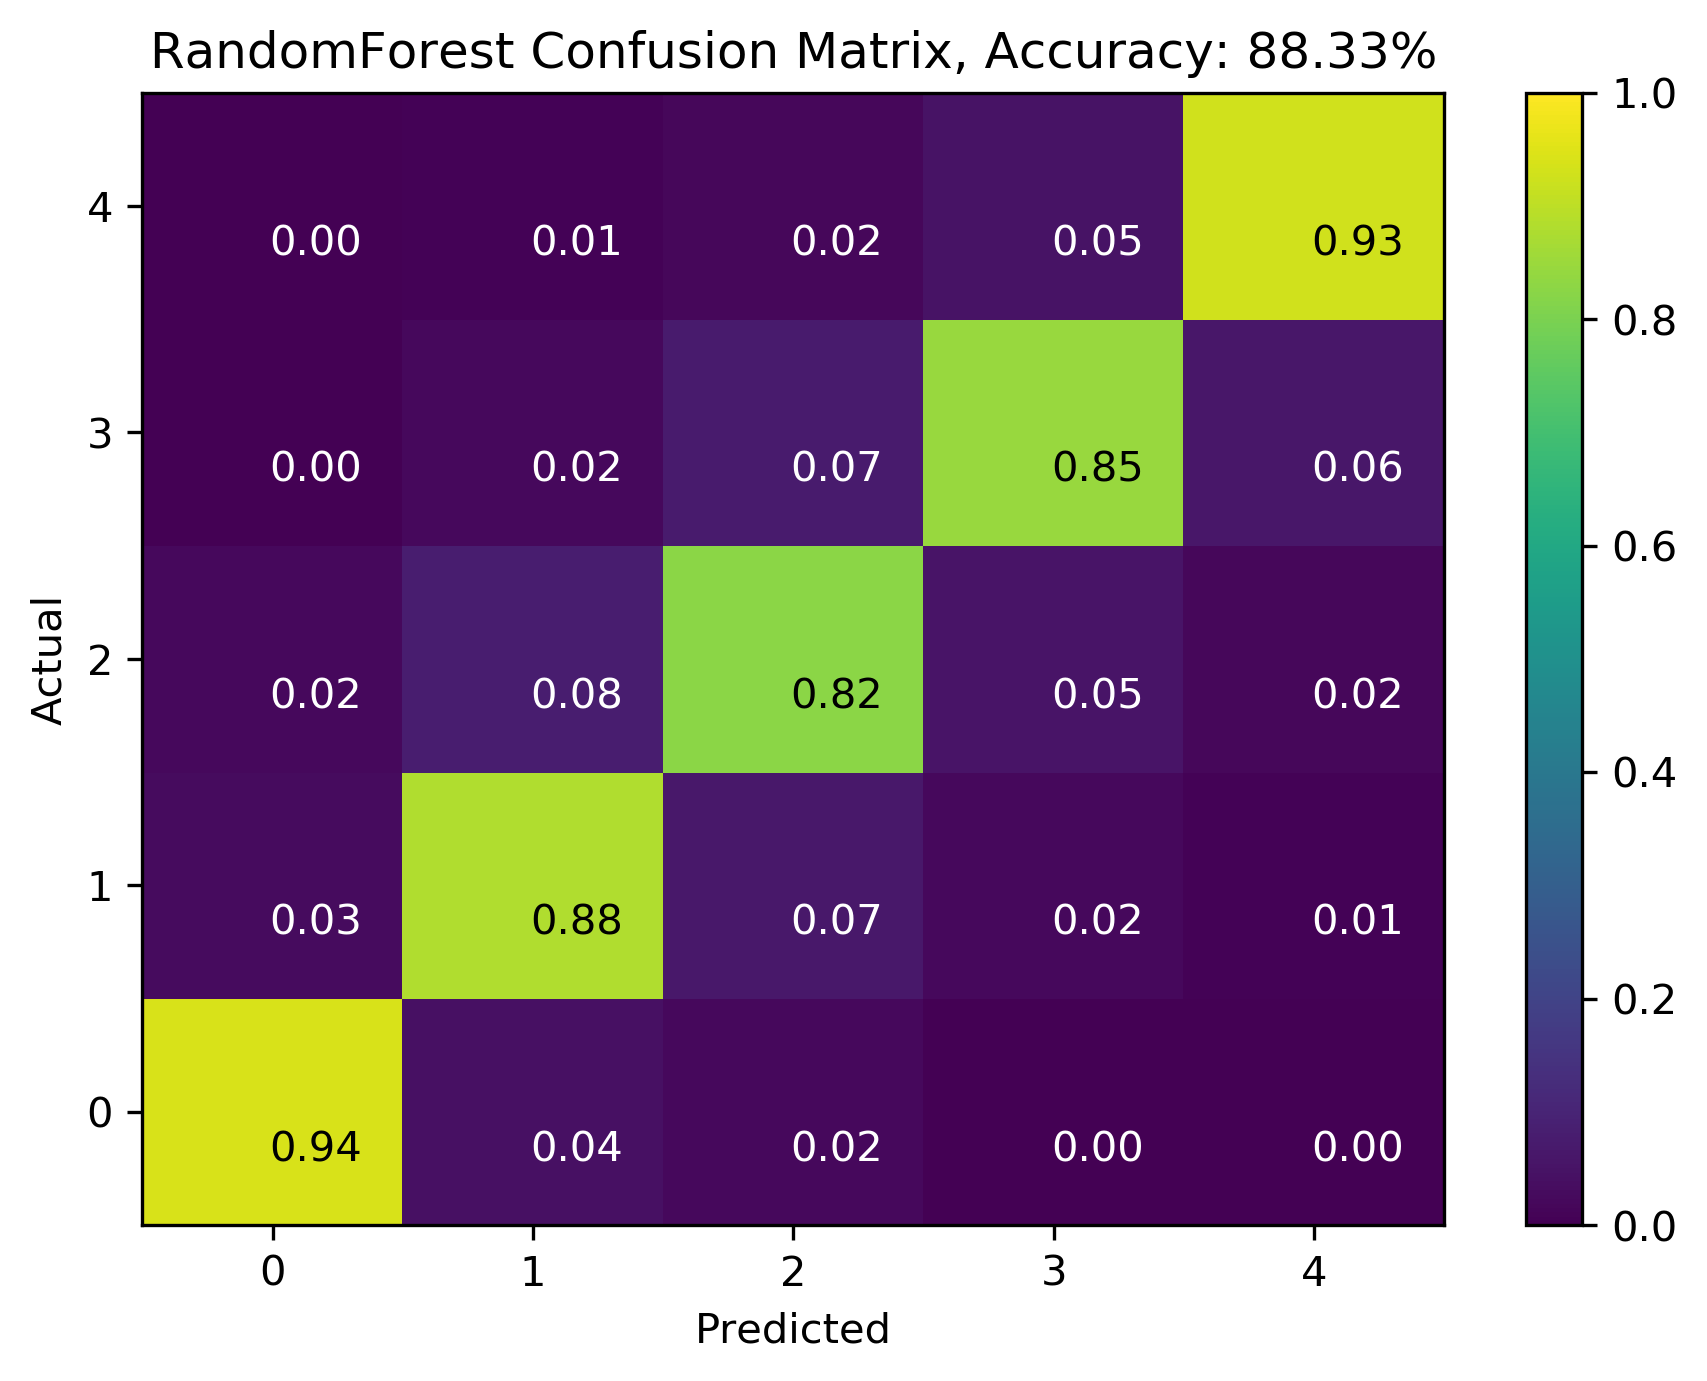
\includegraphics[width=0.5\textwidth]{./plots/RandomForestCM.png}}
\subfloat[] {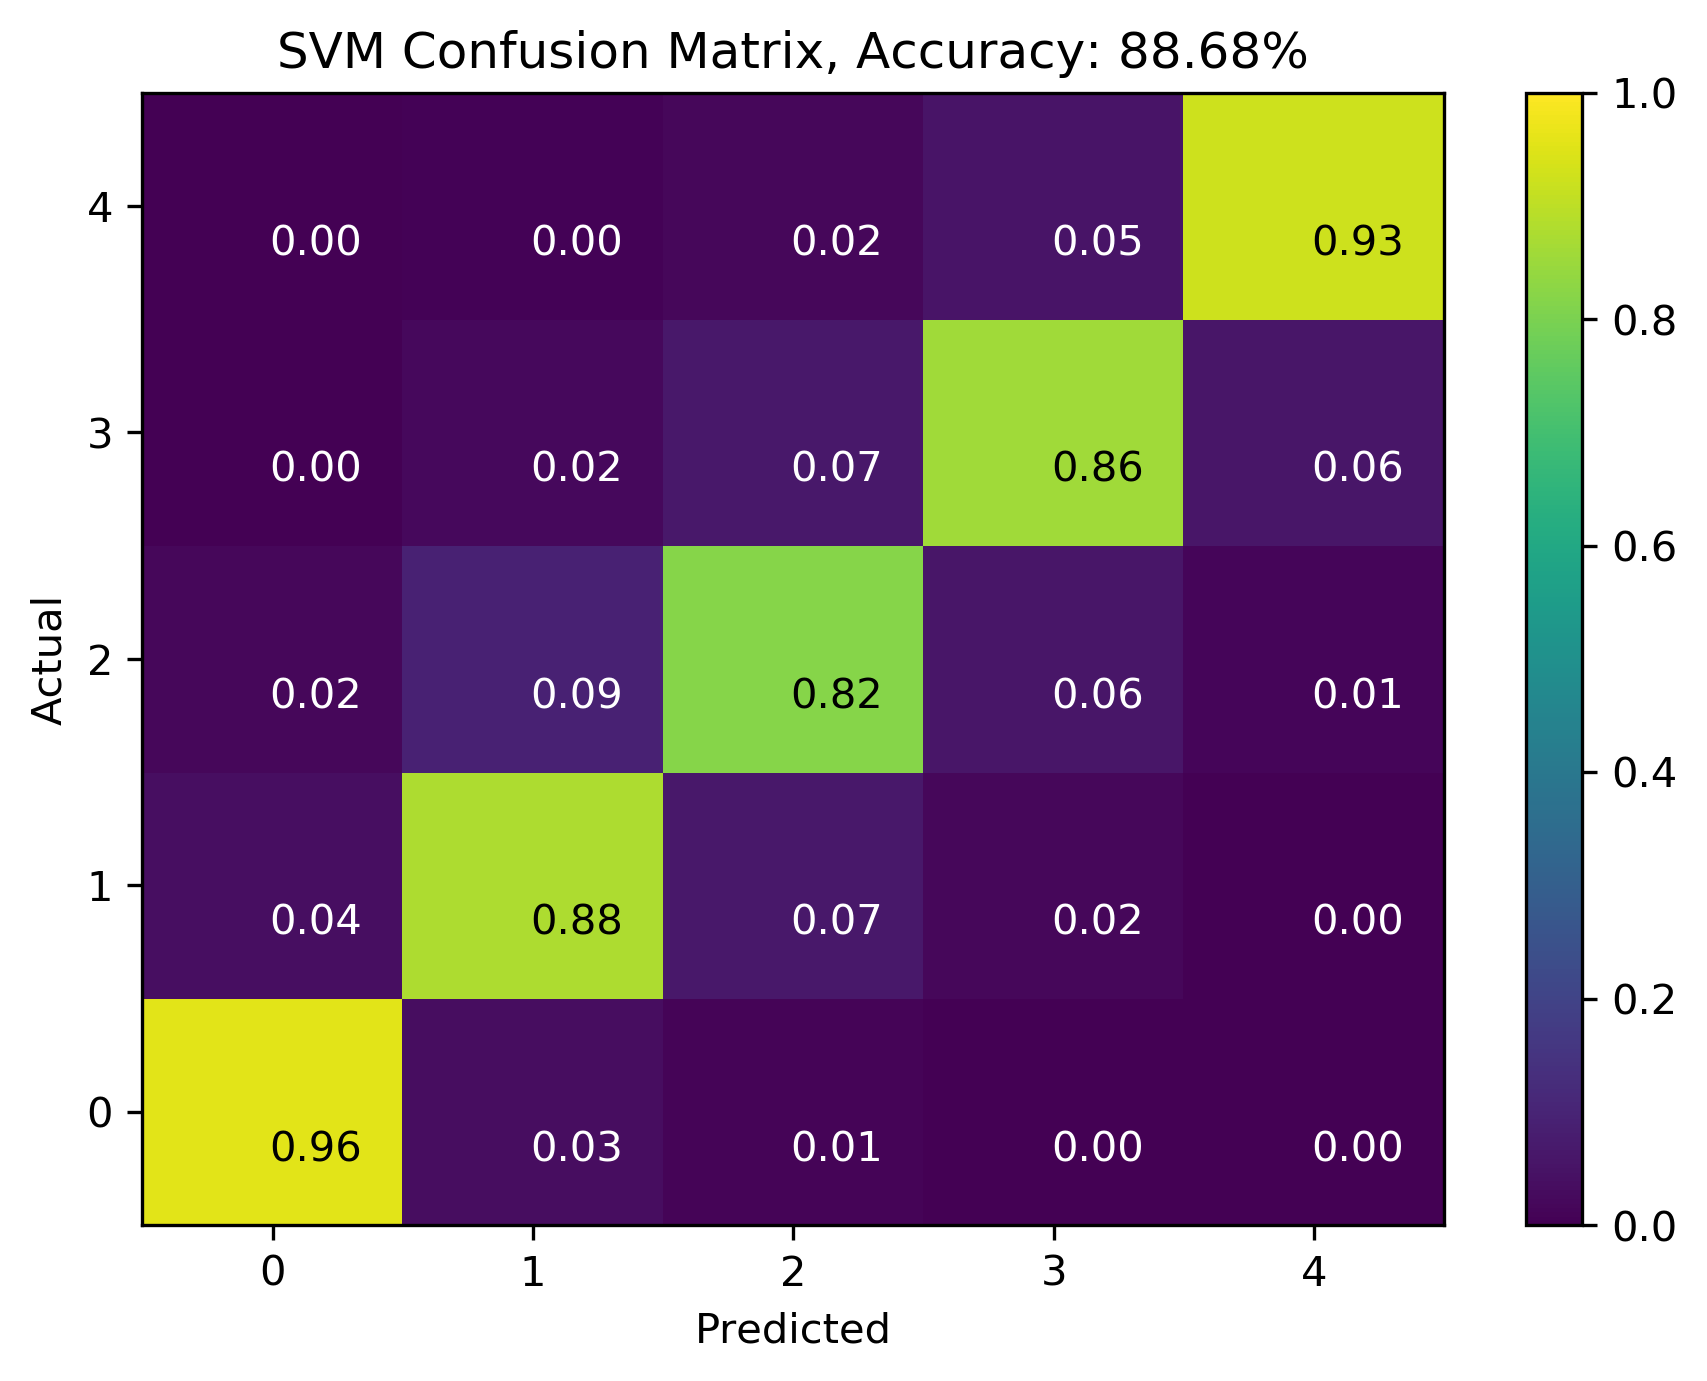
\includegraphics[width=0.5\textwidth]{./plots/SVMCM.png}}
\end{figure}
\vspace*{-1.5cm}
\begin{figure}[H]
\captionsetup[subfigure]{labelformat=empty}
\centering
\subfloat[]{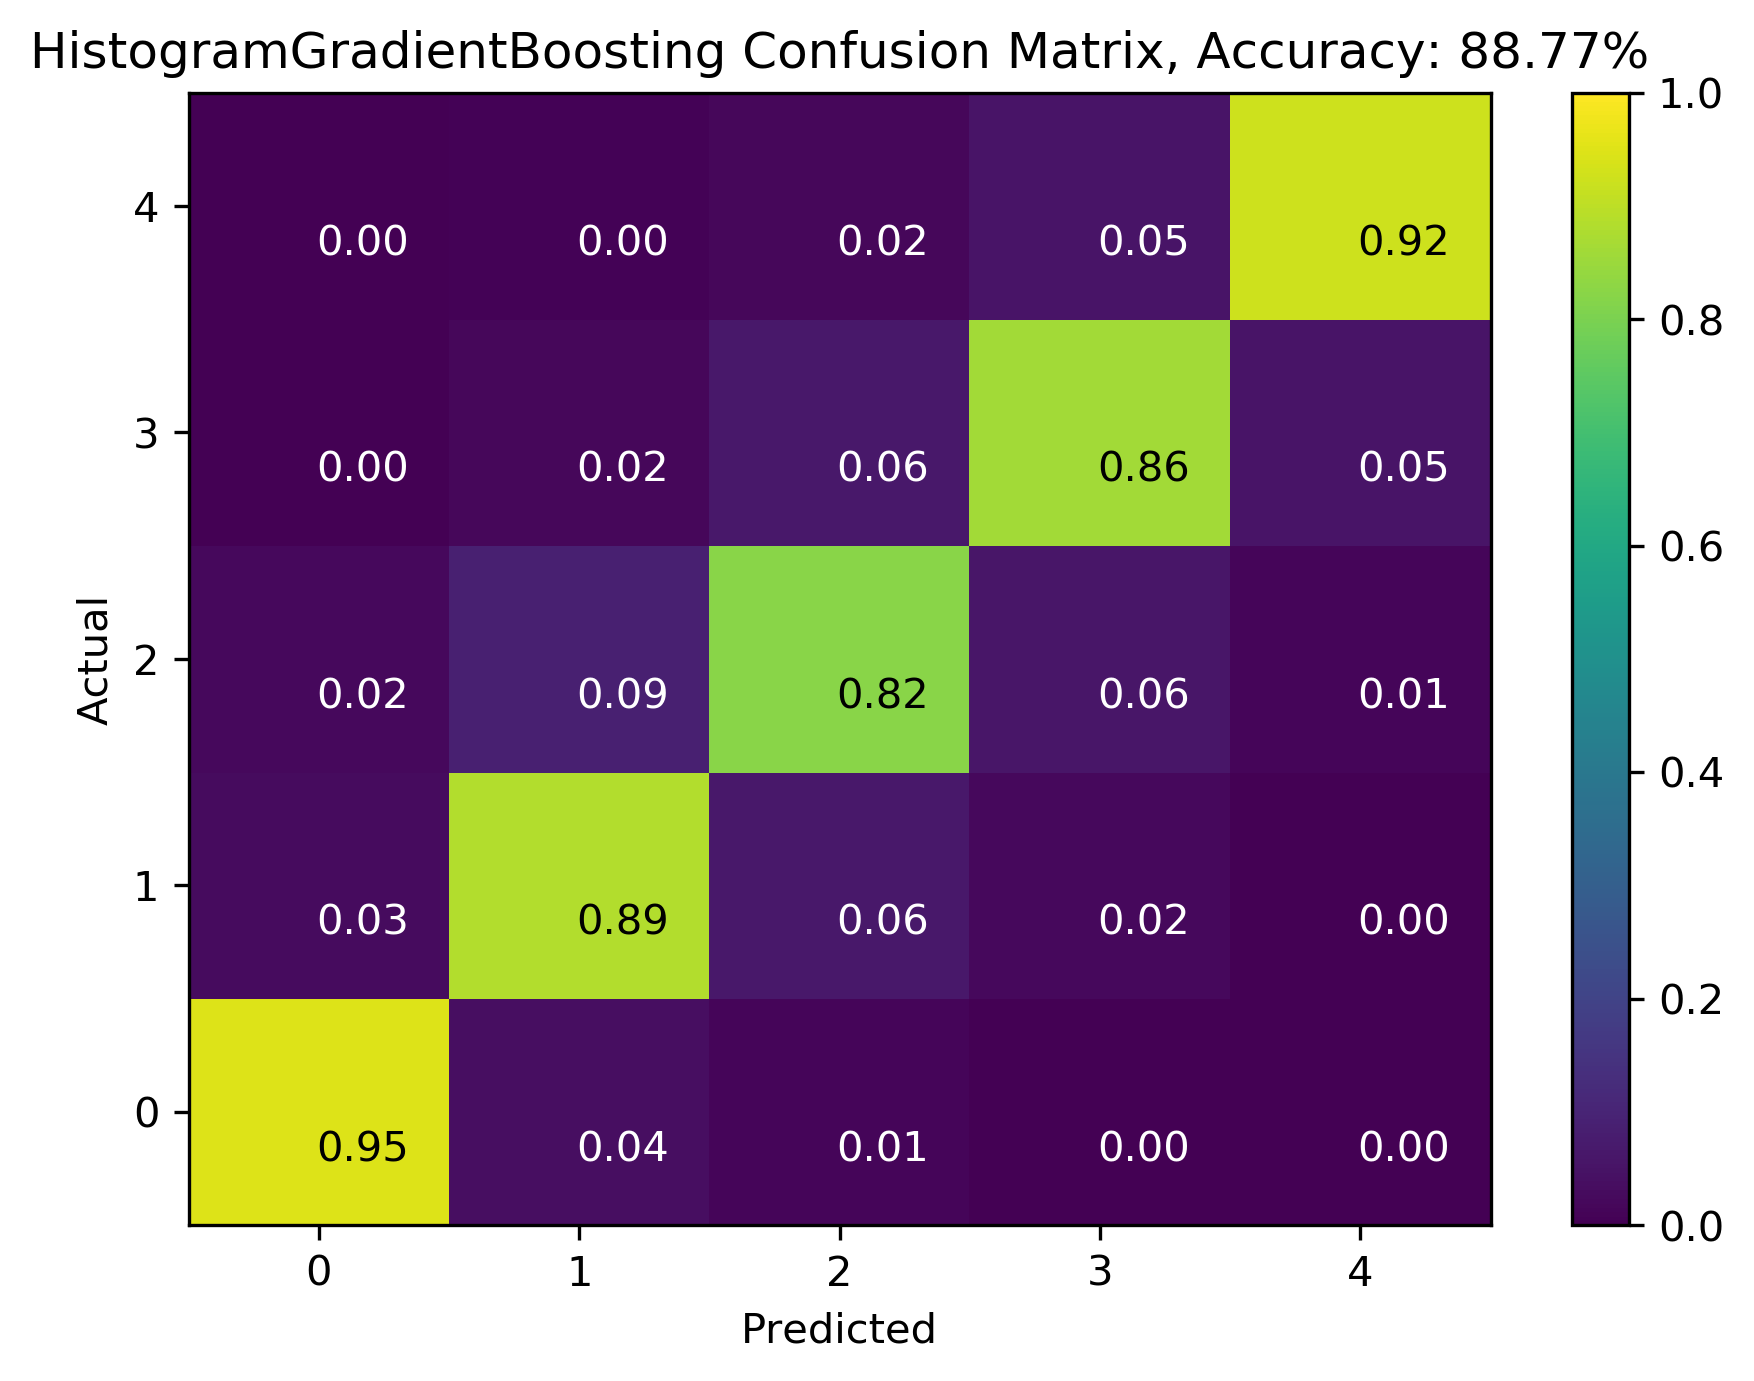
\includegraphics[width=0.5\textwidth]{./plots/HistogramGradientBoostingCM.png}}
\subfloat[] {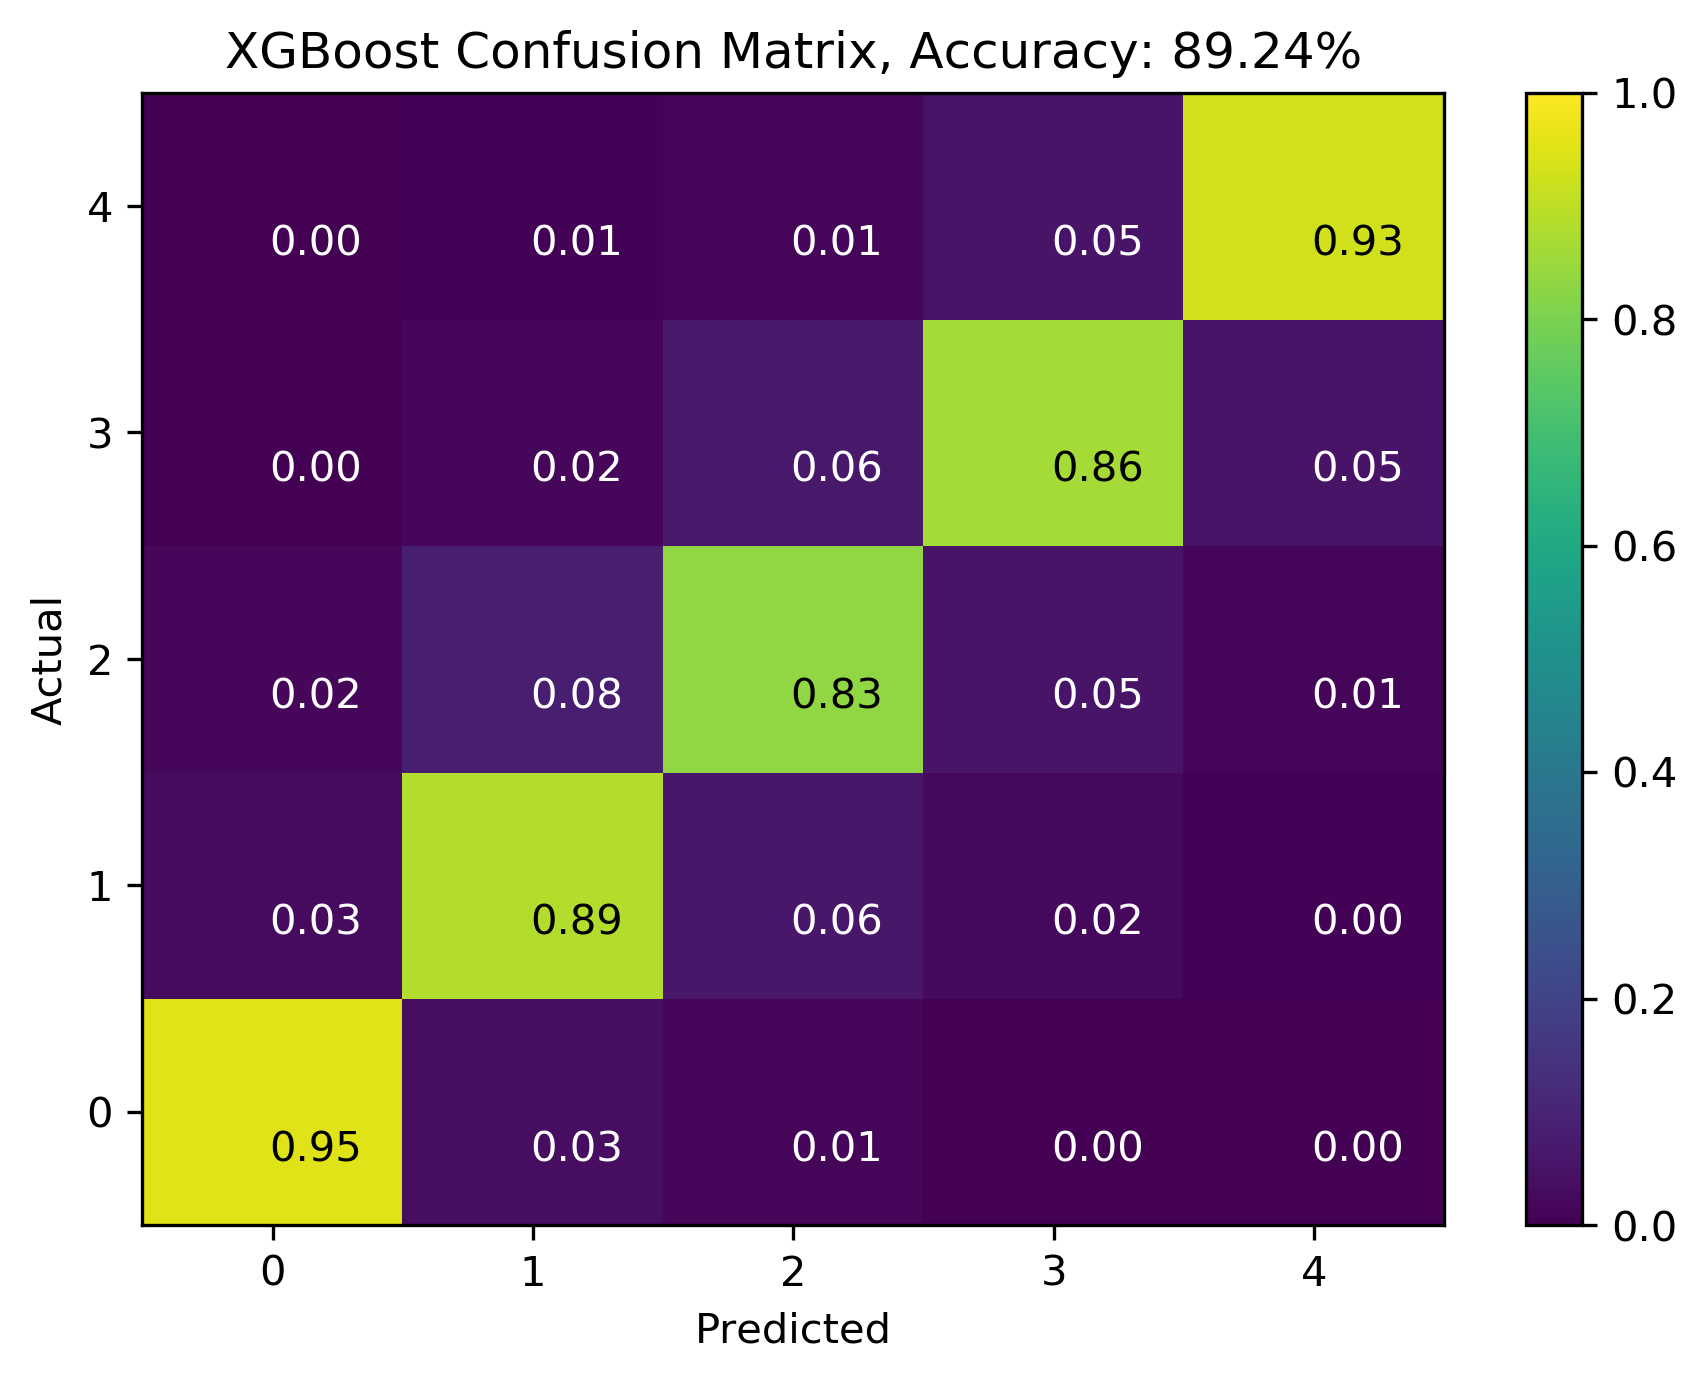
\includegraphics[width=0.5\textwidth]{./plots/XGBoostCM.png}}
\end{figure}
\vspace*{-1.5cm}
The accuracy given by Kaggle is:
\begin{center}
\begin{tabularx}{0.8\textwidth} { 
| >{\raggedright\arraybackslash}X 
| >{\raggedleft\arraybackslash}X | }
\hline
\textbf{Classifier} & \textbf{Accuracy}\\ 
\hline
Random Forest & 88.14\%\\ 
\hline
SVM & 88.78\%\\
\hline
XGBoost & 89.38\%\\
\hline
Histogram-based Gradient Boosting & 89.20\%\\
\hline
\end{tabularx}
\end{center}

From the confusion matrices we can see that for all four algorithms, it is easier to classify class 0 and 4 than other 3 classes. The accuracy to classify 0 and 4 is around 93 percent while it is only 82 percent for class 2. We can also see that the similarity between adjacent classes is relatively greater, for most misclassification rate is contributed by the grids next to the minor diagonals on the matrices.

For random forest, the accuracy will not increase any more when the number of estimators increased to a certain amount, no matter what the other parameters are. However, the accuracy of Hist gradient boosting and xgboost will increase gradually when the learning rate is decreased and n\_estimator is increased.

The specific parameters I tried for each algorithm will be discussed in the following sub-subsection.

\subsubsection{Explanation of your model}
Use GridSearchCV(5 folds) to find the best parameters for each algorithm.

\textbf{Random Forest}
\begin{itemize}
    \item n\_estimators: default value(100), we do not have to tune this parameter since we all know a larger value at least will not make the result worse.
    \item criterion: [gini, entropy], different functions to measure the quality of a split.
    \item max\_features: [auto, log2, 0.25, 0.5, 0.75], number of features to consider when split.
    \item min\_samples\_split: [2, 4, 6, 8, 10], min samples required to split a node.
    \item min\_samples\_leaf: [1, 3, 5], min samples required to be a leaf node.
    \item max\_depth: [20, 40, 60], max tree depth.
\end{itemize}

In total 450 combinations. Best parameter: \{criterion: entropy, max\_depth: 40, max\_features: 0.5, min\_samples\_leaf: 1, min\_samples\_split: 4\}, accuracy: 88.5\%.

\textbf{SVM}
\begin{itemize}
    \item kernel: rbf, image classification is a nonlinear problem so linear kernel was not considered. And the poly kernel was not considered for its low efficiency according to \href{https://www.kdnuggets.com/2016/06/select-support-vector-machine-kernels.html}{this blog}.
    \item C: [0.01, 0.1, 1, 5, 10, 15, 20, 25, 30, 35], regularization parameter.
\end{itemize}

In total 10 combinations. Best parameter: \{C: 35\}, accuracy: 88.56\%.

\textbf{Hist Gradient Boosting}
\begin{itemize}
    \item learning\_rate: default value(0.1)
    \item max\_iter: default value(100), lower the learning rate and increase max iteration will almost always improve the result, so I did not tune these two parameters.
    \item max\_leaf\_nodes: [35, 37, 39, 41], max leaves for each tree.
    \item min\_samples\_leaf: [22, 24, 26, 28], min samples per leaf. Since the training set is large, I tried values greater than the default value(20).
\end{itemize}

In total 16 combinations. Best parameter: \{max\_leaf\_node: 41, min\_samples\_leaf: 24\}, accuracy: 88.83\%

\textbf{XGBoost}

Following the instruction on \href{https://www.analyticsvidhya.com/blog/2016/03/complete-guide-parameter-tuning-xgboost-with-codes-python/}{this blog}, I tuned these parameters step by step.

Step 1:
\begin{itemize}
    \item max\_depth: [3, 5, 7, 9, 15], max depth of a tree, typical value 3-10.
    \item min\_child\_weight: [1, 3, 5], min sum of weights of all observations required in a child.
\end{itemize}

Step 2:
\begin{itemize}
    \item gamma: [0, 0.1, 0.2, 0.3, 0.4], regularisation parameter.
\end{itemize}

Step3:
\begin{itemize}
    \item sub\_sample: [0.6, 0.7, 0.8, 0.9], subsample ratio, to prevent overfitting.
    \item colsample\_bytree: [0.6, 0.7, 0.8, 0.9], subsample ratio of columns when constructing a tree.
\end{itemize}

Step 4:
\begin{itemize}
    \item reg\_alpha: [0, 1e-5, 1e-2, 0.1], l1 regularisation parameter, the greater, the more conservative the model will be.
\end{itemize}

In total 15+5+16+4=40 combinations. Best parameters: \{max\_depth: 15, min\_child\_weight: 1, gamma: 0, subsample: 0.8, colsample\_bytree: 0.9, reg\_alpha: 0\}, accuracy: 89.31\%.

XGBoost has the best performance among all 4 algorithms.

\subsubsection{ROC Curve}
ROC plots of the four algorithms are shown below, AUC is calculated in the plots' legend.
\begin{figure}[H]
\captionsetup[subfigure]{labelformat=empty}
\centering
\subfloat[]{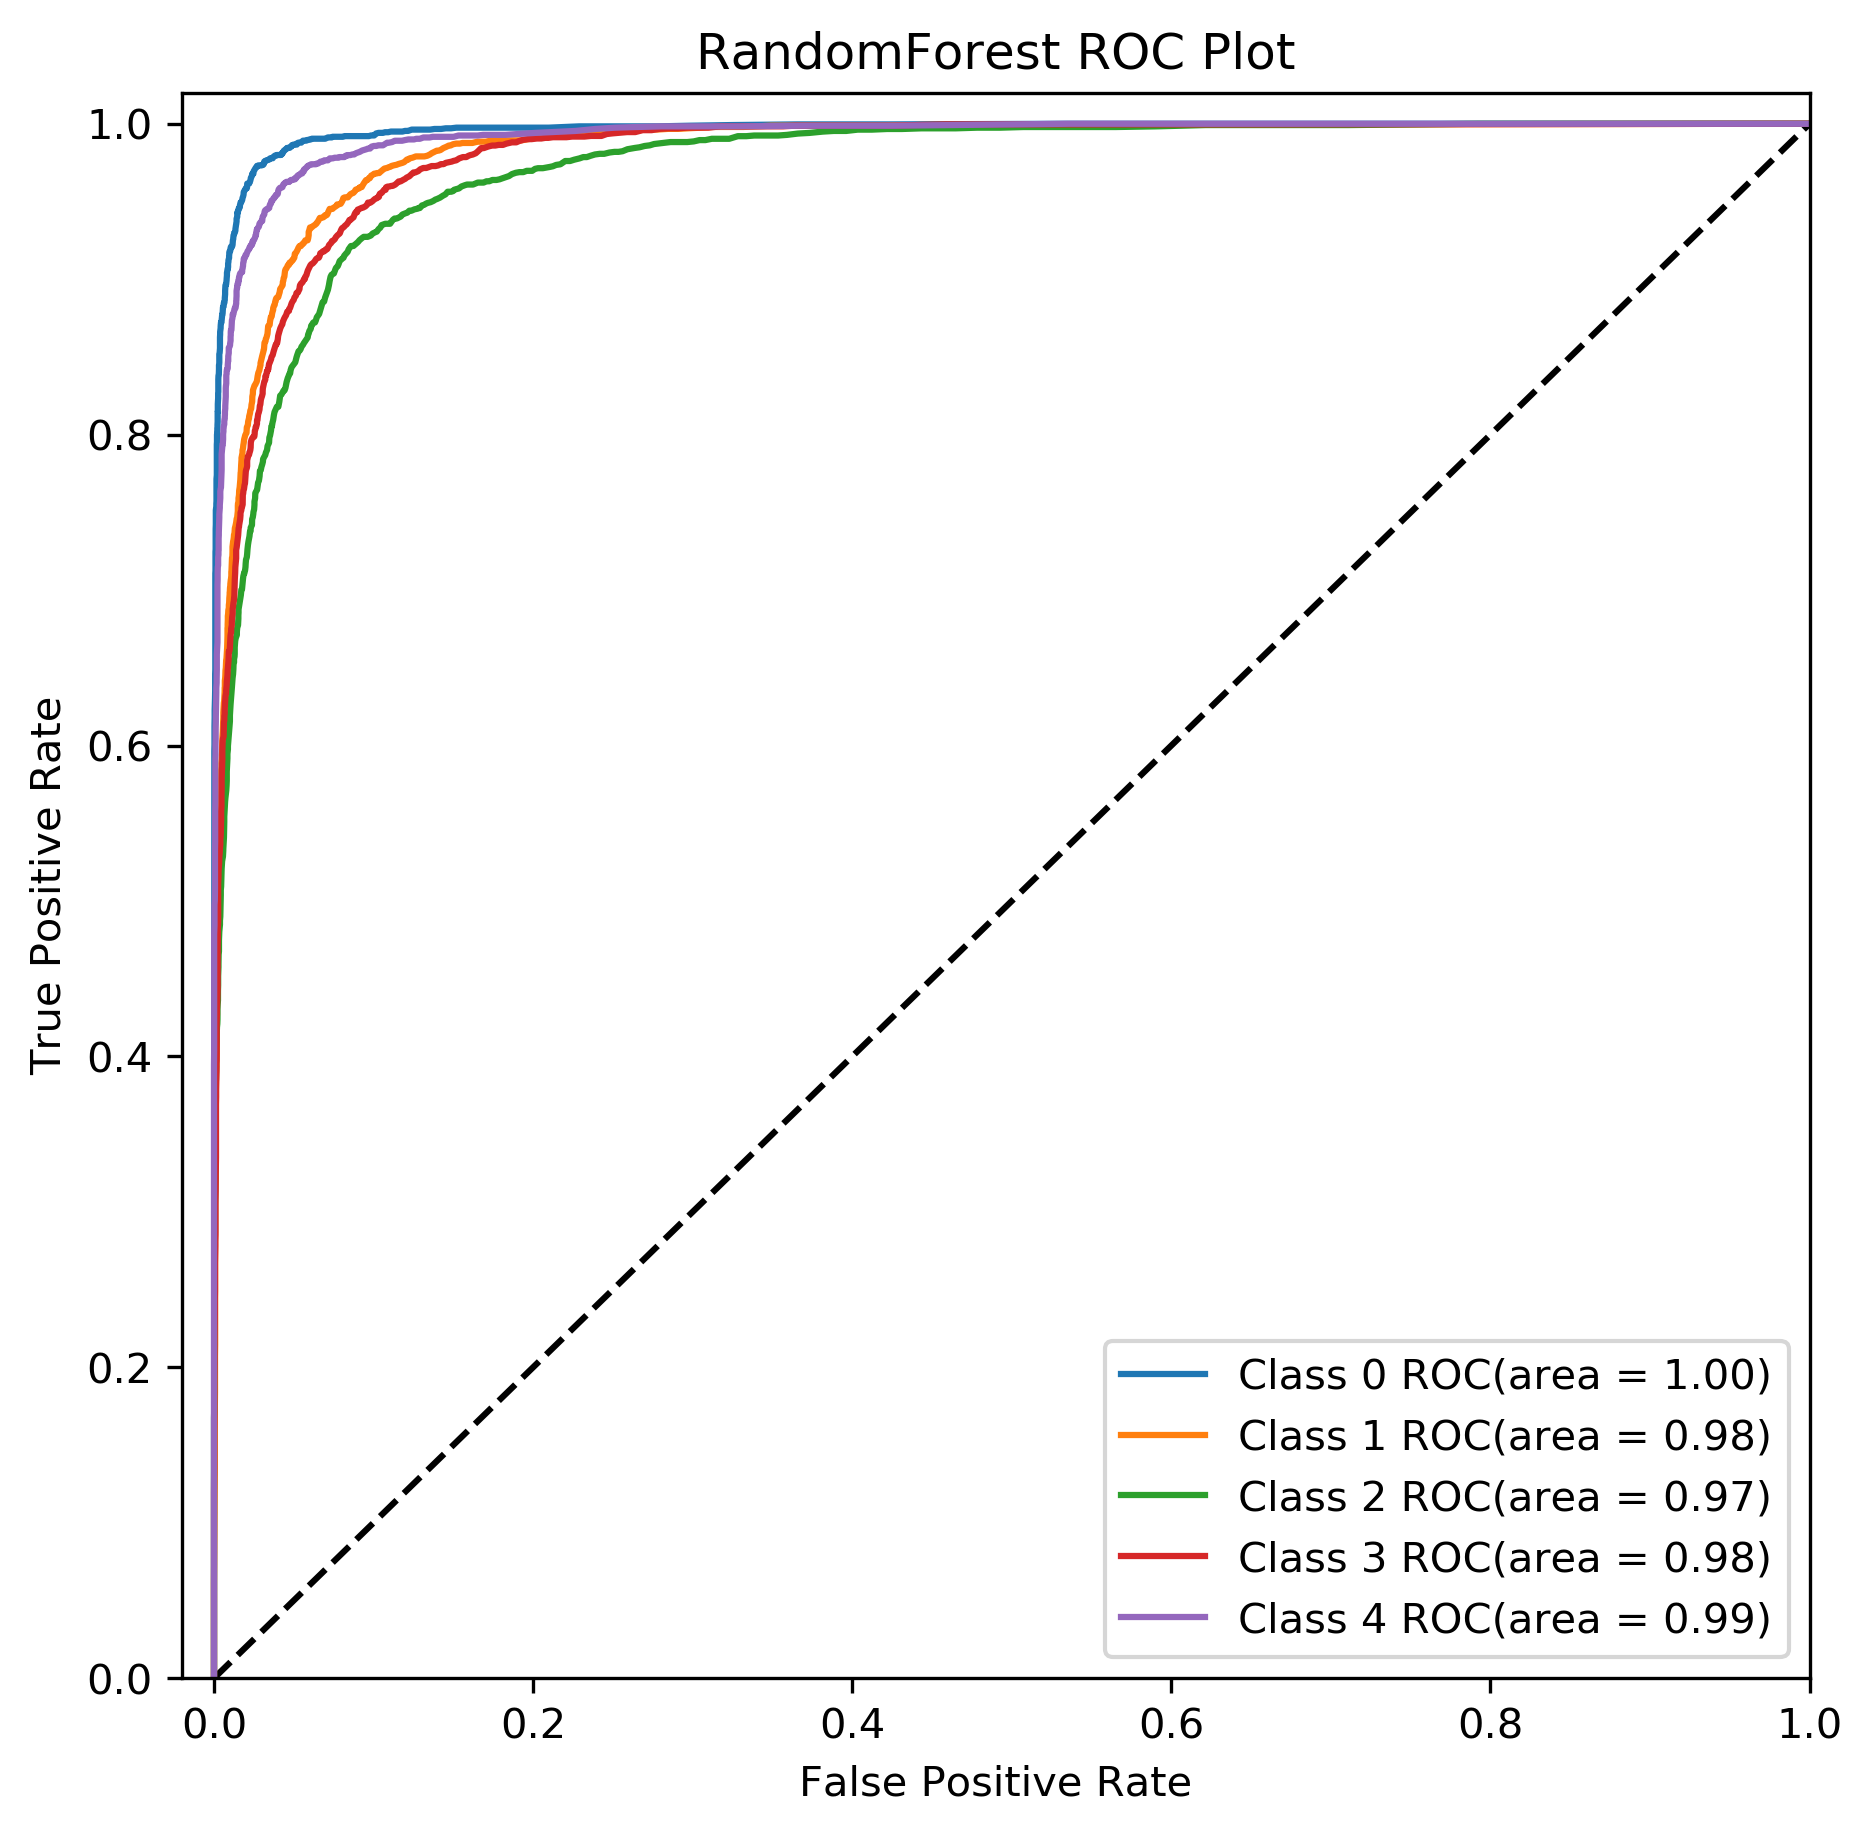
\includegraphics[width=0.5\textwidth]{./plots/RandomForest_ROC.png}}
\subfloat[] {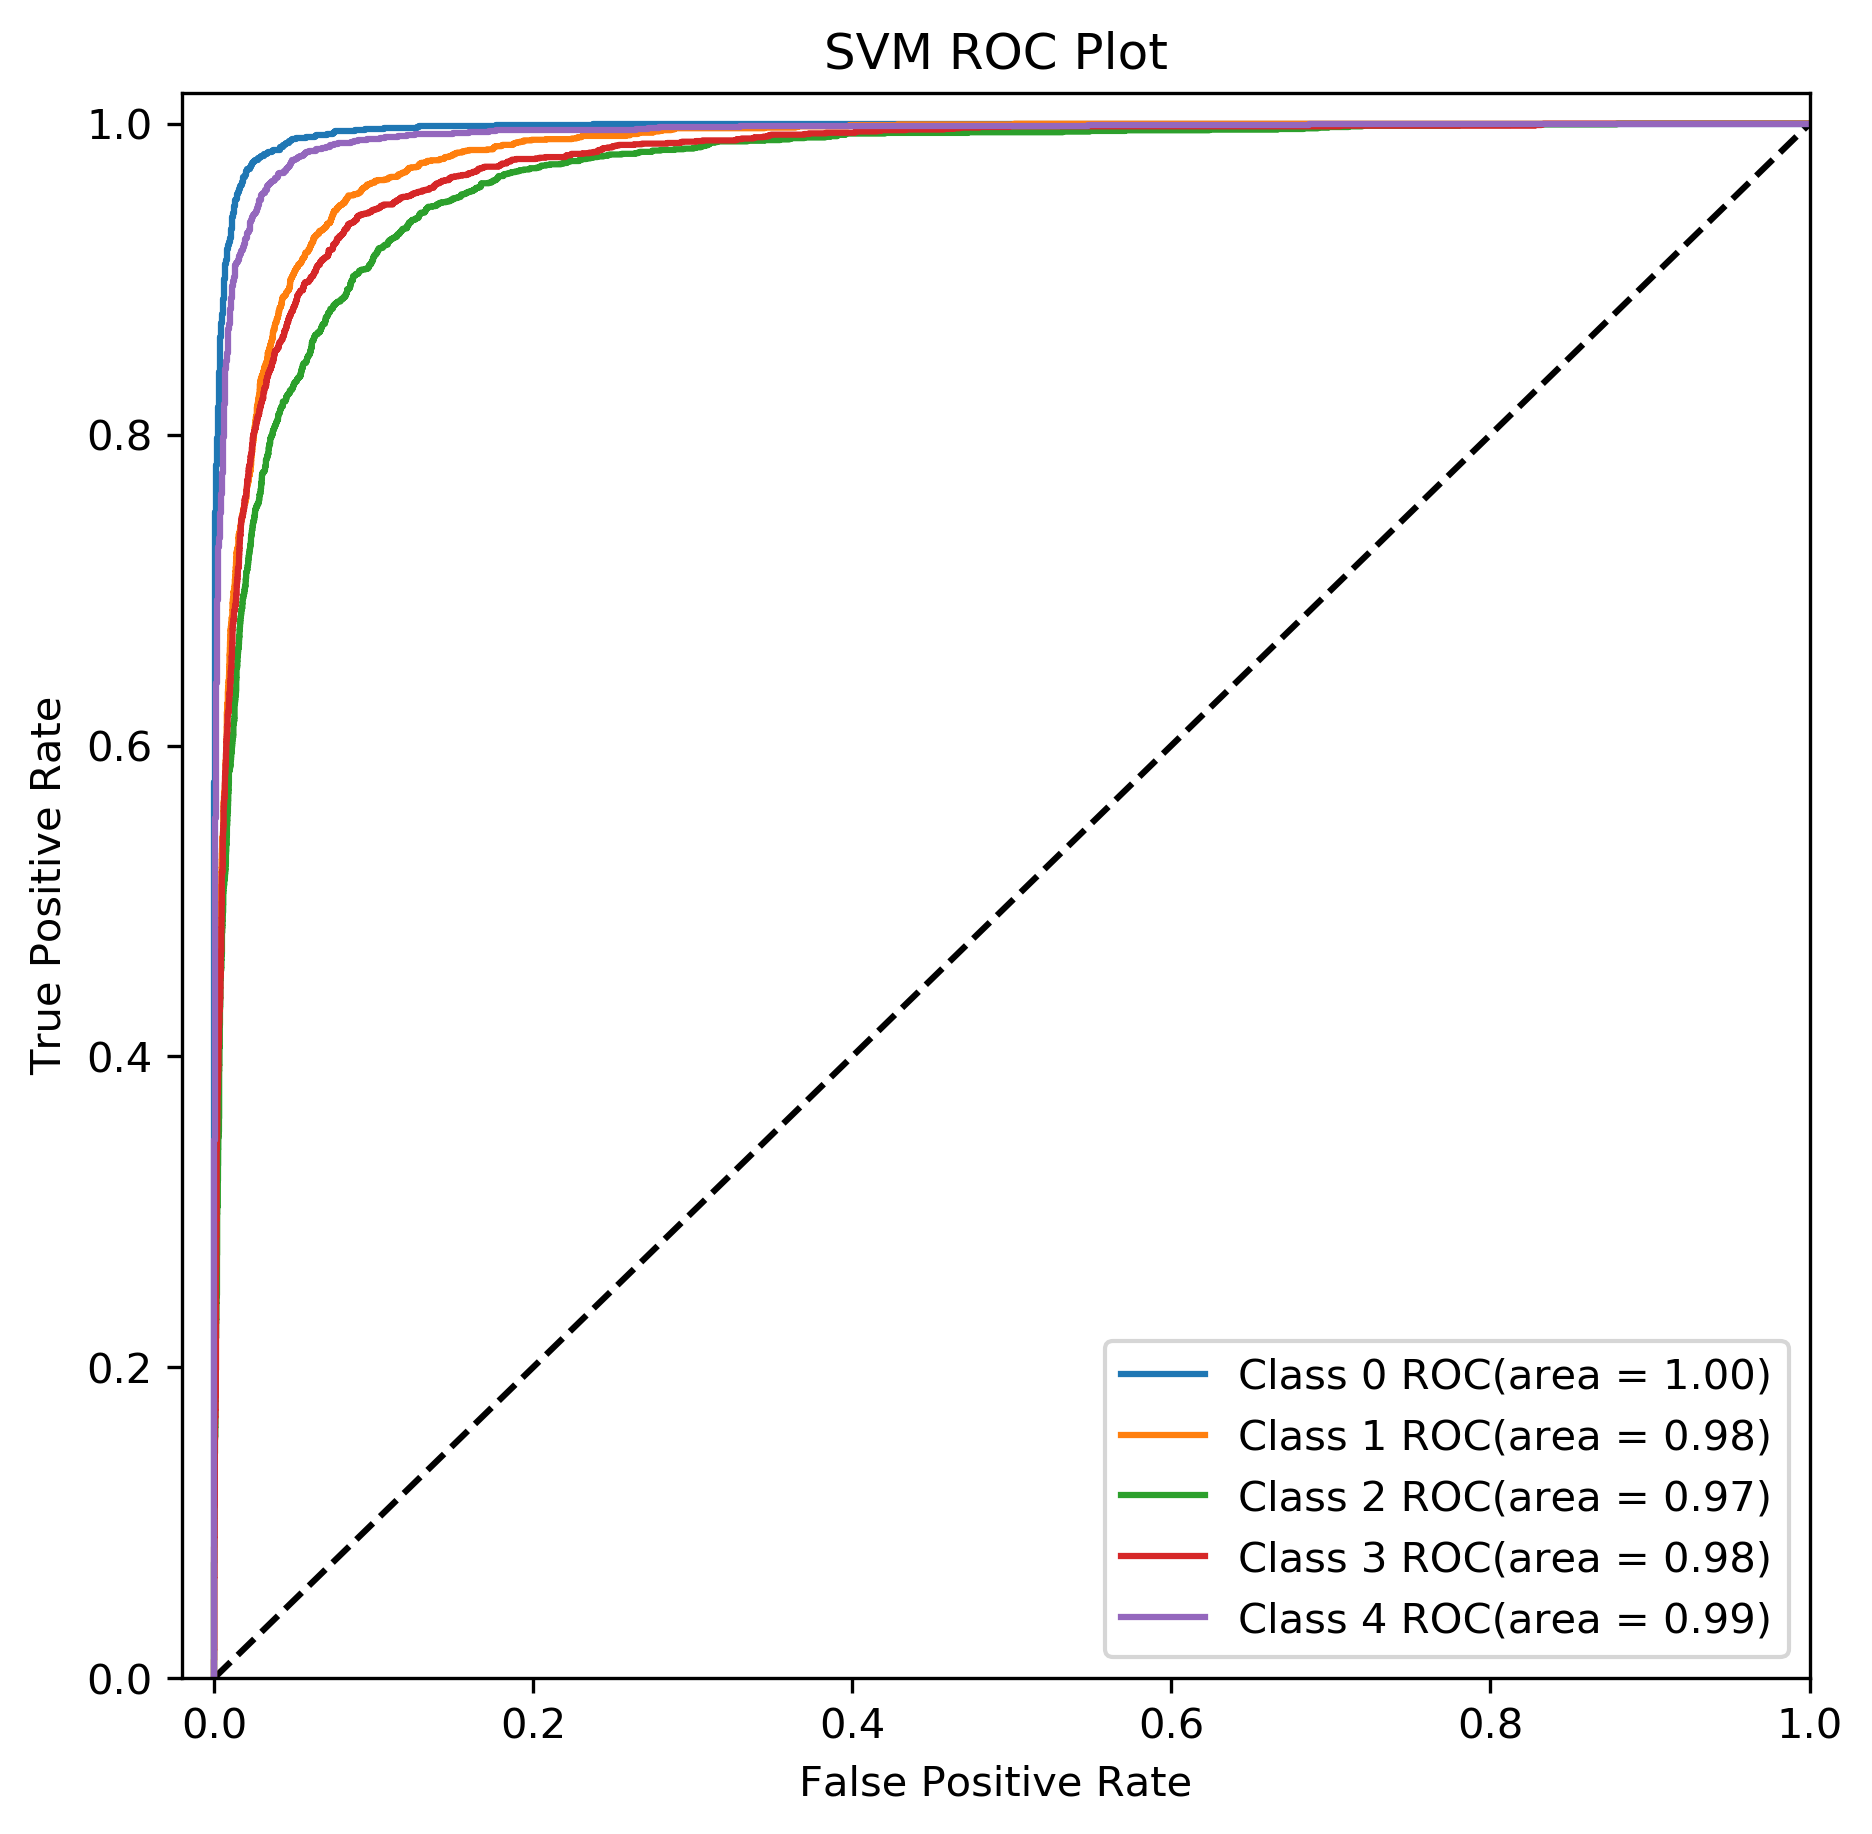
\includegraphics[width=0.5\textwidth]{./plots/SVM_ROC.png}}
\end{figure}
\vspace*{-1.5cm}
\begin{figure}[H]
\captionsetup[subfigure]{labelformat=empty}
\centering
\subfloat[]{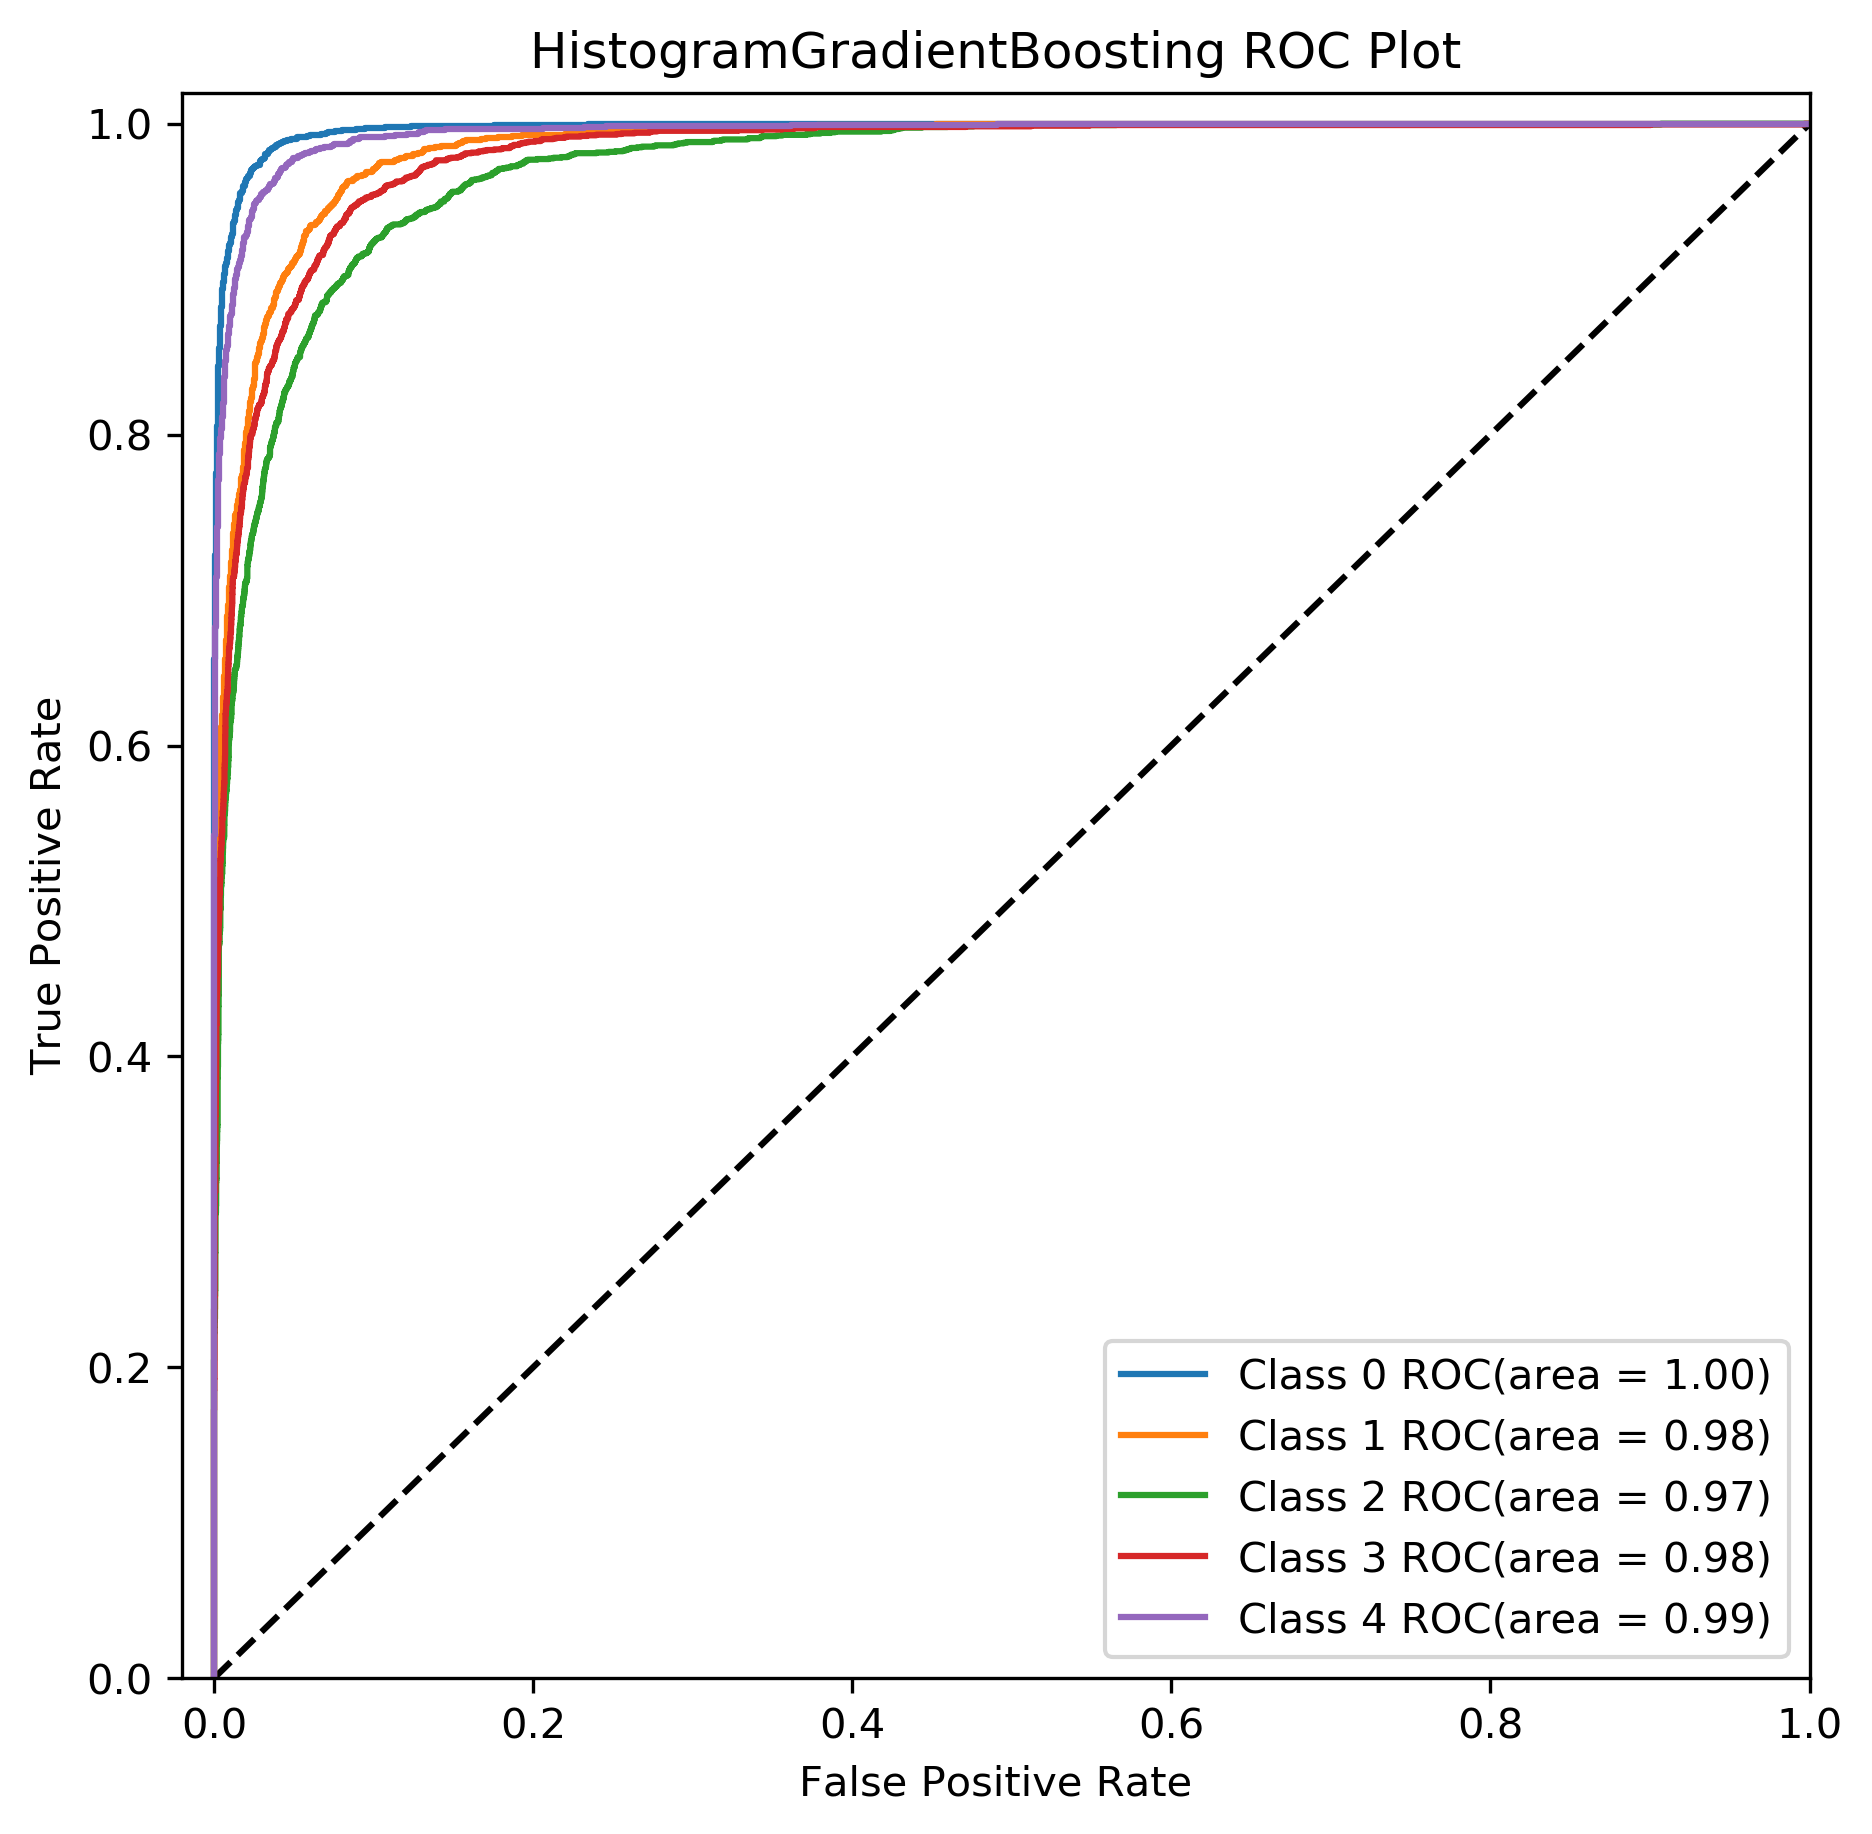
\includegraphics[width=0.5\textwidth]{./plots/HistogramGradientBoosting_ROC.png}}
\subfloat[] {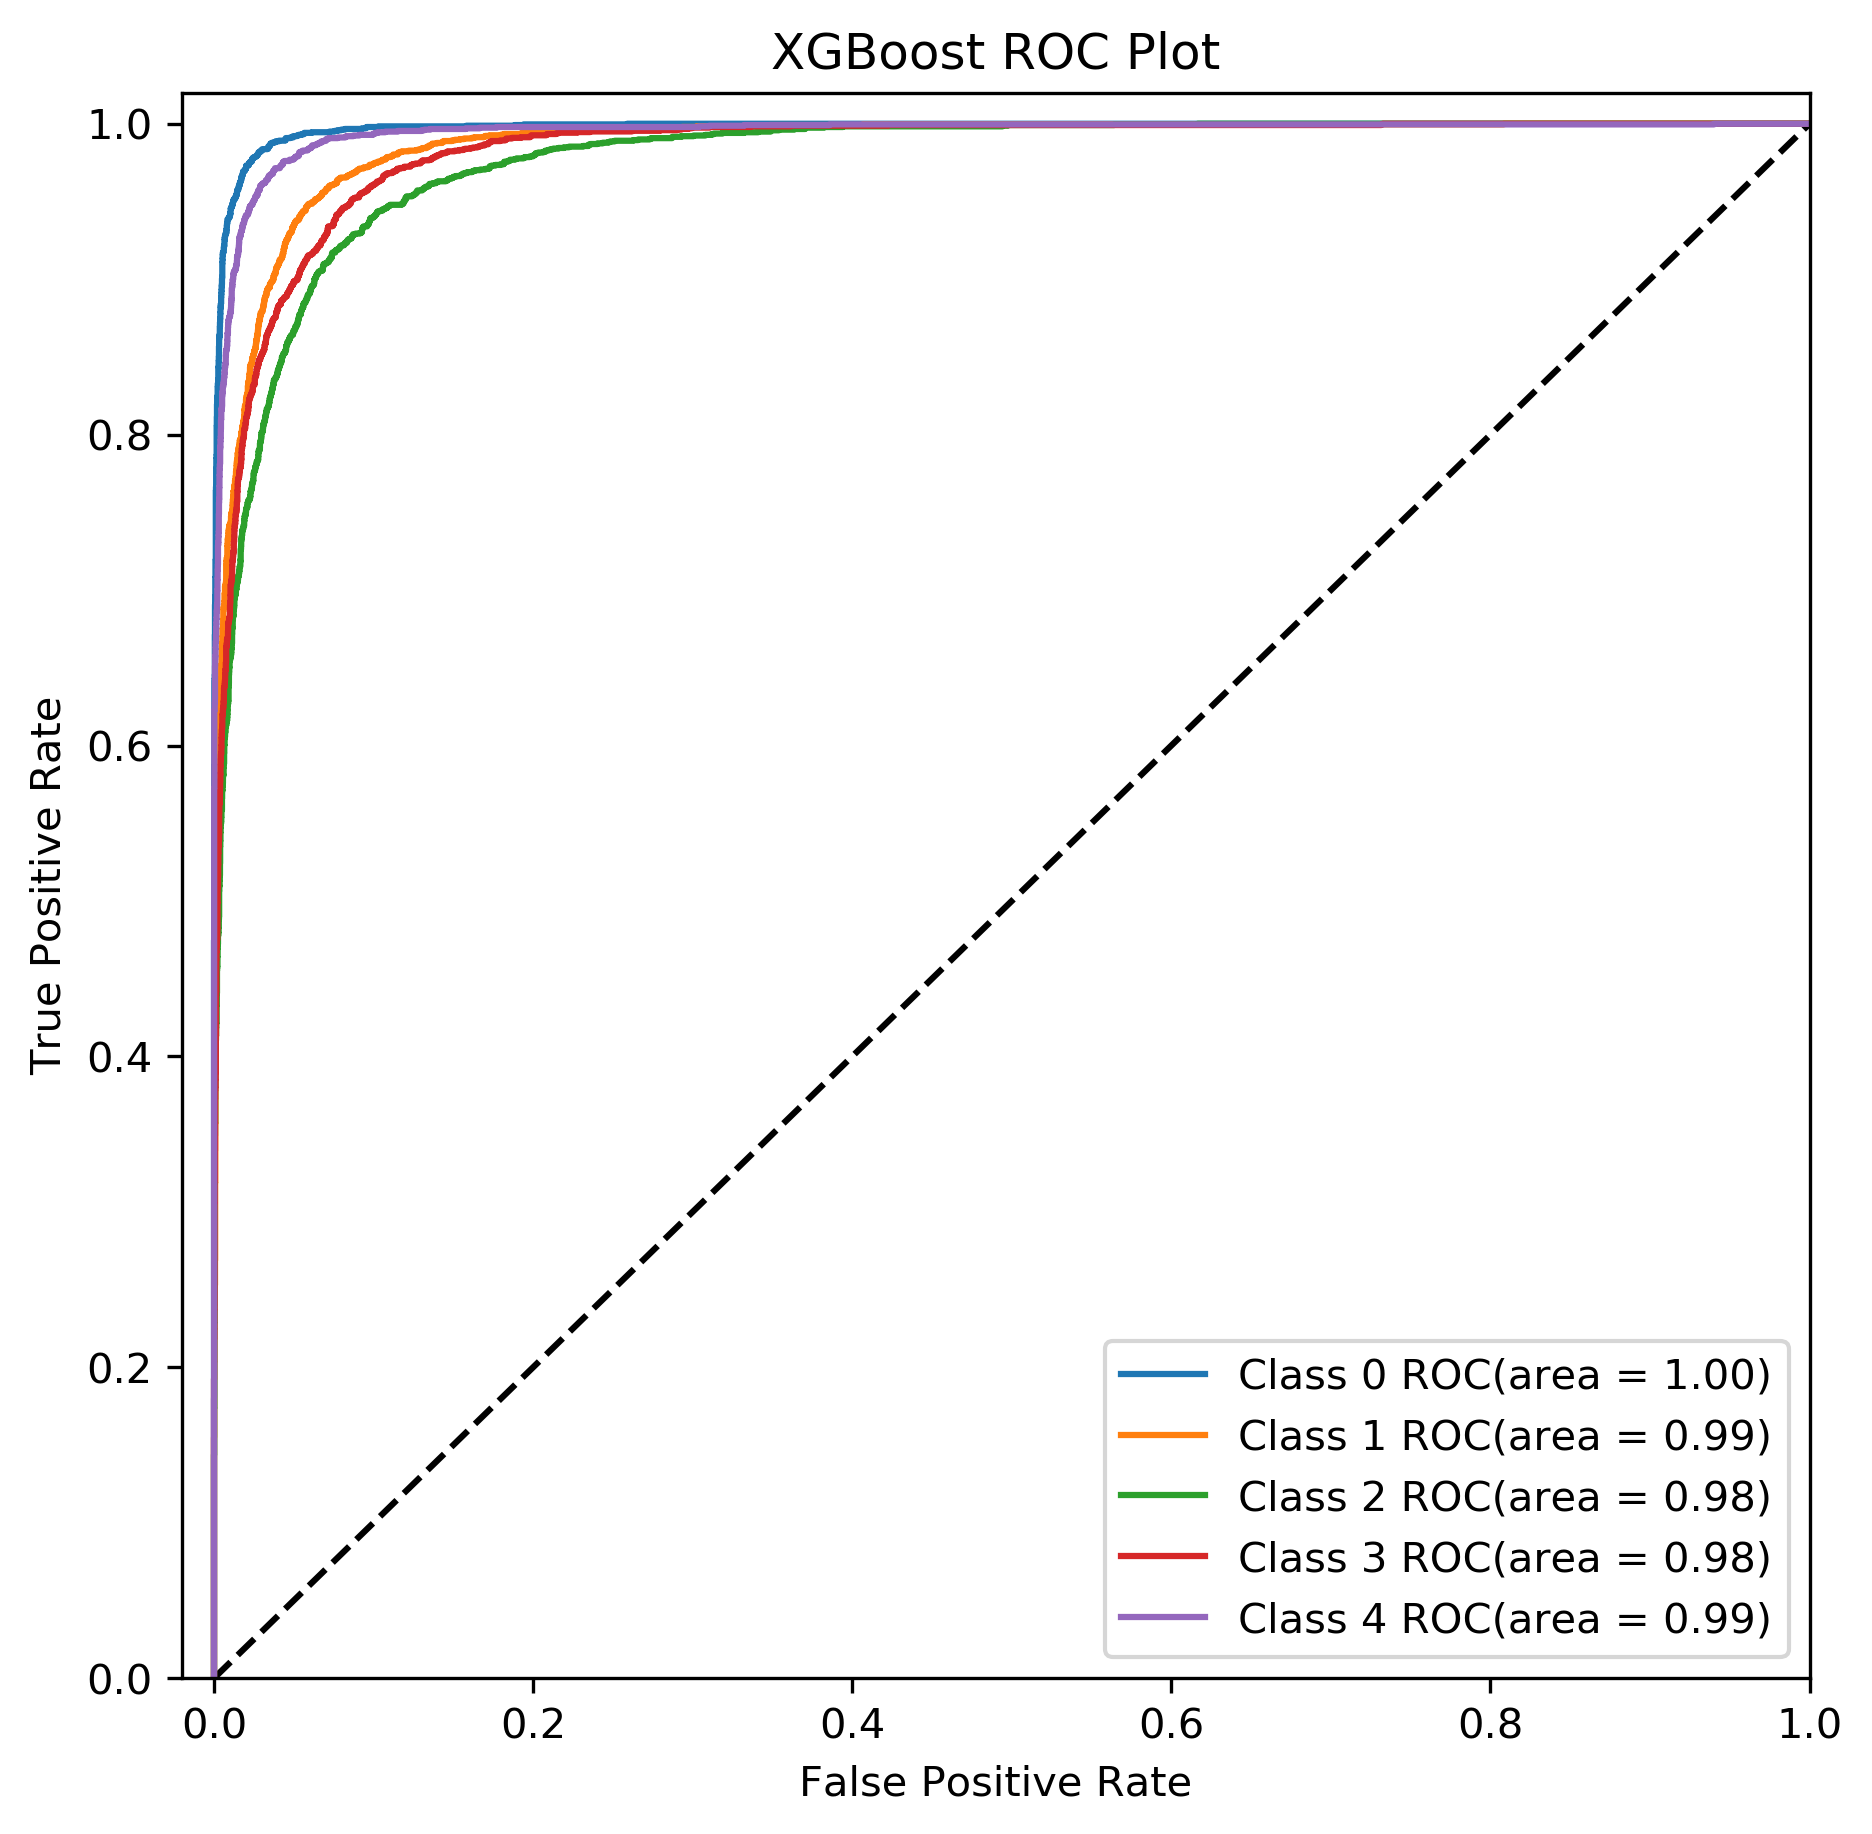
\includegraphics[width=0.5\textwidth]{./plots/XGBoost_ROC.png}}
\end{figure}
\vspace*{-1.5cm}
The ROC curve was plotted using one-vs-all methodology since this is a multi-class model. So there are 5 lines in each plot, each line represents the ROC curve of one class versus the other classes.

We can learn from the plots that the classifiers performed fairly good on this dataset, as the AUC is close to 1 for all curves. For example, there is 98 percent of chance that the random forest model will be able to distinguish class 1 from other classes. 

We also know that the difficulty to separate each class is class 2 $>$ 3 $>$ 1 $>$ 4 $>$ 0.

\subsubsection{Evaluate your code with other metrics on the training data and argue for the benefit of you approach}

\end{document}